\section{Background}
\label{sec:background}

\subsection{RDMA}

\begin{figure*}[t]
    \centering
    \begin{subfigure}{0.3\linewidth}
        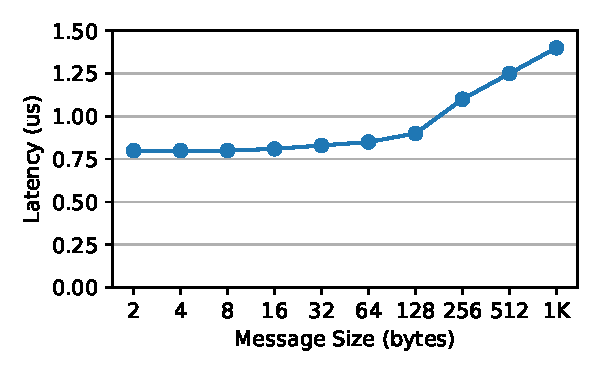
\includegraphics[width=0.99\linewidth]{fig/rdma_latency.pdf}
        \label{fig:rdma_latency}
        % \caption{}
    \end{subfigure}.
    \begin{subfigure}{0.3\linewidth}
        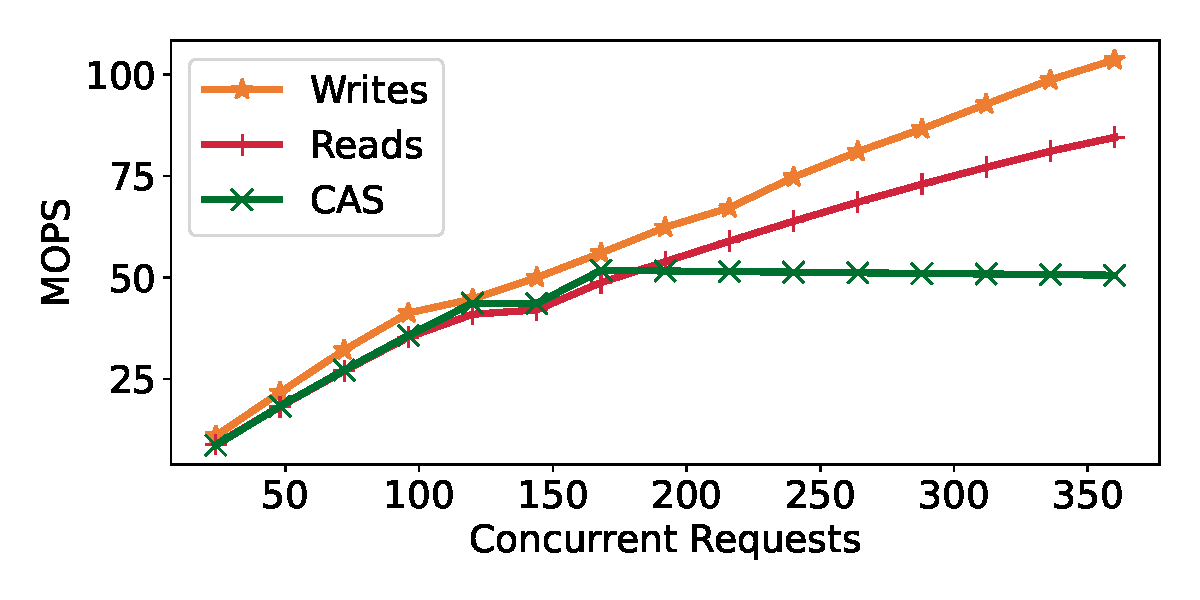
\includegraphics[width=0.99\linewidth]{fig/rdma_concur.pdf}
        % \label{fig:optimistic_failures}
        % \caption{}
    \end{subfigure}
    \begin{subfigure}{0.3\linewidth}
        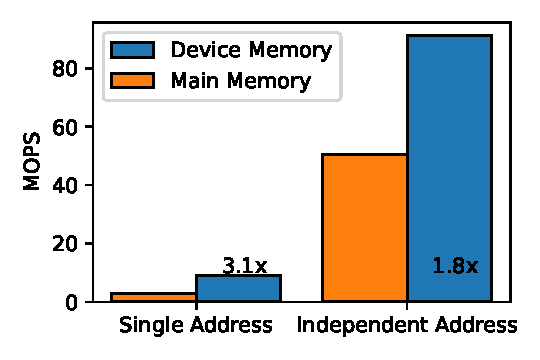
\includegraphics[width=0.99\linewidth]{fig/rdma_cas_throughput.pdf}
        % \label{fig:optimistic_failures}
        % \caption{}
    \end{subfigure}
    \vspace{-1em}
    \caption{
    \textbf{(a)} CX5 RDMA latency vs message size~\cite{rdma-latency}
    \textbf{(b)} RDMA operation scalability
    \textbf{(c)} Compare and swap performance. Device memory vs main memory.
    }
    \label{fig:rdma-benchmarks}
\end{figure*}

RDMA is a networking technology which allows client machines
to directly access the memory of a remote server. RDMA is an
enabling technology for memory disaggregation as
\textit{memory servers} do not need any computation
resources (save setting up the RDMA memory initially). RDMA
is designed for extremely high throughput and low latency.
Bandwidth capabilities of RDMA NICs have increased
disproportionately to their latency improvement. The
bandwidth difference between CX3 and CX7 NICs is 10$\times$ and yet
intra-rack round trips of small RDMA packets has only shrunk
by around 1.5$\times$. Comparatively bandwidth is cheaper than
latency. Figure~\ref{fig:rdma-benchmarks}(a) shows the tradeoff
between NIC to NIC round trips times on CX5 RDMA NICs for
write operations. All packets up to 128 bytes have
comparable round trip latencies, and packet sizes must grow
to above 1K before the latency cost of a large packet exceeds the
cost of two round trips for smaller packets. \textbf{In a network
with surplus bandwidth if single large messages can be used
to achieve the work of two dependent smaller messages system
latency can be improved.}

One-sided RDMA verbs (read, write, atomic) are used to
access remote memory without any memory side computation.
One-sided verbs require RDMA reliable connections which
guarantee in-order delivery of operations enabling dependent
operations to be issued in batches. Operation throughput is
not equivalent across all verbs. Reads and writes scale
approximately linearly, however atomic operations suffer
from throughput bottlenecks at approximately half the
throughput~\cite{design-guidelines,sherman}.
Figure~\ref{fig:rdma-benchmarks}(b) shows the scalability of
these operations on CX5 NICs for 64 bit operations.

The cause of RDMA atomic throughput bottlenecks is mostly
due to PCIe round trips to host memory. NICs are forced to
use complex internal locking schemes which inspect in flight
requests across queue pairs to ensure that no dependent
operations execute concurrently. Vendors have provided small
amounts on-device memory which does not suffer this
limitation~\cite{device-memory}. Device memory access is
lower latency in general as it avoids the PCIe round trip,
and much faster for locking as the critical section is
executed entirely on the NIC~\ref{fig:rdma-benchmarks}(c)
shows the relative performance of CAS operation on device
memory vs host memory. Lock request on a single address are
3x higher throughput, and independent lock requests scale at
nearly the same rate as read and write requests.

RDMA operations are known to have limitations~\cite{prism},
pointer deference, memory allocation, and the scope of CAS
operations are the most debated. Due to fixed width CAS
operations, and no support for multi-CAS, RDMA based
algorithms using optimistic concurrency can only update
single 64-bit values atomically. \textbf{Vendors have provided
masked CAS operations~\cite{rdma-masked-cas} to set multiple
bits independently, this however is not a general solution
as it still demands data locality for items being
independently updated.}


\subsection{RDMA Key-Value Stores}

Many projects have used RDMA to accelerate key-value
stores~\cite{farm,erpc,herd,mica,pilaf,cell,faast,storm,memc3}.
RDMA verb use is a matter of contention among these systems.
Typically reads are lock-free and made directly to remote
memory, while writes use two-sided verbs and are coordinated
by the server side CPU.
%%
Far memory key-value stores have no server side CPU and must
therefore use client side synchronization to achieve
serializablity~\cite{rolex,fusee,clover,sherman,ford,race}.
These systems make use of RDMA atomic verbs for
serialization. However, the use of the atomics is highly
dependent on the key-value stores under lying data
structure.

\textbf{Data Structures} - The underlying data structures of
far-memory key value stores has a large impact on the
system's performance. To perform fast reads CPU colocated
systems have used cuckoo and hopscotch
hashing~\cite{pilaf,herd,cuckoo,hopscotch}. While these
structures have fast predictable reads, they have a large
number of updates required for
insertions~\cite{pilaf,cuckoo-improvements,memc3}. These
large critical sections are amplified by far memory access
times and lead to performance bottlenecks when acquiring
locks. Recent work on remote memory data structures have
opted for optimistic concurrency~\cite{clover,race,ford}.
This strategy comes at the cost of additional round trips to
first learn up-to-date information about the remote
structure, and to ensure that the optimistic operation
completed successfully.

\textbf{Cuckoo hashing} is a hash table which delivers constant-time reads. It uses two hash functions to determine two
possible locations at which any hashed item can reside. When
reading both locations are queried. If the item is not
found, it is not in the table. On insert, the item is placed
in the first location it hashes to. If that location is full
the item in that location is evicted and kicked to it's
second location.  This process happens iteratively for many
items. The sequence of displaced keys on an insert is called
a ~\textit{cuckoo-path}~\cite{cuckoo-improvements}. When a
loop occurs in a cuckoo path the insert fails and the table
is resized. Fill factors for cuckoo hashes can be improved
by using associative buckets for each hash index, and
shortening cuckoo paths by using BFS rather than radom
search~\cite{cuckoo-improvements}.